\chapter{Phideus-Beacon Convergence}

\epigraph{\emph{The probes do not agree; they become answerable to one another.}}{}



\section{Two perspectives on the same hypothesis}


The central hypothesis of HIT, stated at its widest scale, is that harmonic or proportional organization matters for the structuring of information, for the stability of material systems, and for the ways living and symbolic processes hold together. Part V approaches that hypothesis through two probes built from very different materials. Phideus begins from paired datasets in which two domains register the same event, trains dual encoders and projection heads, compares descriptor-guided arms against explicit baselines, and asks whether ratio-based descriptions reorganize cross-modal representation. Beacon begins from the generation of sustained harmonic fields in physical space, calibrates those fields through resonant instruments and situated listening, and asks whether immersion in such conditions modifies bodily and experiential states. The conjunction with Personal Myth Projection adds a third site of observation: a structured therapeutic setting in which the presence of a harmonic field may matter for the accessibility and handling of deep psychic material.

Taken together, these probes open three distinct experimental registers. Phideus works in the computational register, where the question is whether proportional descriptions reorganize latent geometry under controlled variation. Beacon works in the physiological and experiential register, where the question is whether a sustained harmonic field modifies states, responses, and conditions of resonance in lived situations. PMP plus Beacon works in the psychological register, where the question is whether that same type of field changes the dynamics by which difficult symbolic material becomes accessible, stays open, and is later integrated. The registers are different, the instruments are different, and the vocabularies are different. What they share is a commitment to the same family of hypotheses: that harmonic organization carries structural consequences.

The asymmetry of maturity between the branches is real and informative. Phideus has closed positive evidence in its first completed front: replicated gains, causal controls, and measurable geometric reorganization. Beacon has a coherent device lineage, repeated observations, working protocols, and an experimental program that is already generating discriminating questions. PMP plus Beacon adds an established field practice with structured observation, interviews, before-and-after tests, and therapeutic follow-up across multiple applications. The open work there concerns formalization, comparison, and explanation. Convergence therefore works through mutual feedback and retroactive reshaping: heterogeneous probes reshape what becomes askable and legible in one another.


\section{The feedback loop: how each probe informs the other}


The two probes share a theoretical commitment and already feed each other in concrete ways. Phideus contributes a descriptor taxonomy, an explicit baseline-first discipline, and an adversarial culture of evaluation. The descriptor families developed there, from local interval structure to linear ratio profiles and harmonic amplitude summaries, extend naturally into the experiential setting. They can operate as harmonicity sensors for Beacon devices, helping tune a field, compare variants, or discriminate between natural, perceptual, and deliberately non-ratio controls. The same is true of the logic of comparison. The distinction between baseline and descriptor-guided arm, so central in Chapter 11, translates directly into Beacon design: one needs a field, a matched comparison, and a way of reading the delta rather than the isolated condition.

Beacon feeds Phideus through a different route. Corazofono practice suggests that each body presents a specific resonant organization and that this organization matters for how a sustained field is received. That observation pushes computational work toward descriptors that preserve individual spectral identity rather than washing it out into population averages. More broadly, Beacon keeps returning the computational branch to the room, the body, and the transduction chain. What Phideus measures in latent space remains connected to the fact that real signals come from situated bodies in real acoustic ecologies. That pressure widens the field of relevance of its descriptors and keeps its metrics tied to the environments from which those signals arise.

The feedback becomes more legible once PMP is added as a third vertex. Personal Myth Projection contributes a vocabulary of process that retrieval metrics and autonomic traces do not articulate by themselves. It asks a different question: what kind of access, symbolic descent, confrontation, or integration becomes more available under a sustained harmonic field? In that sense, the combined PMP-Beacon setting becomes another discriminating instrument, one able to say something about temporal process, psychic handling, and the structure of difficult material once the field is present.

The first direct experimental convergence between the two main probes occurs in the program's third phase, centered on Lissajous figures. Phideus approaches that object through synthetic generation with exact parametric ground truth. Beacon approaches it through analog capture, using physical resonance instruments, optical readout, and the multi-agent exploration architecture described in Chapter 12. Once the same proportional relations appear in both pipelines, a genuinely new question becomes available: whether the organization learned from synthetic data transfers to patterns captured from the physical world. The question treats both probes as two ways of reaching the same object and asks whether the structure detected on one side survives the passage to the other.

\begin{figure}[ht]
\centering
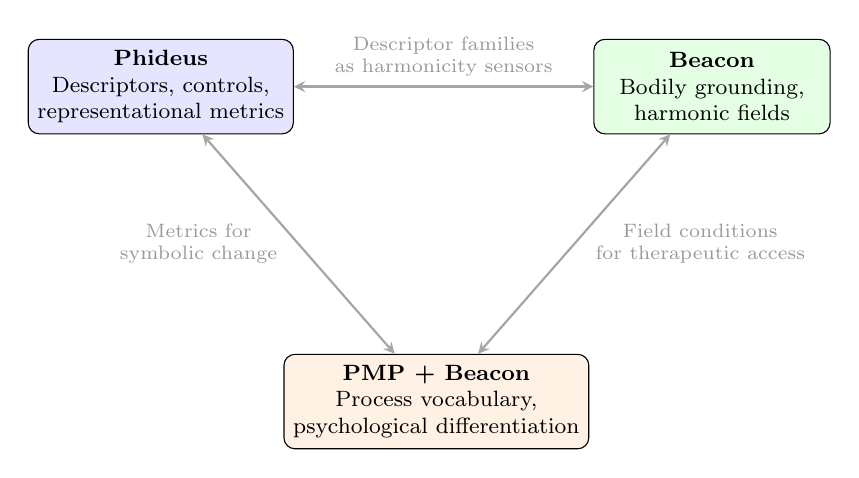
\begin{tikzpicture}[
    vertex/.style={rectangle, draw, rounded corners=4pt, minimum width=3cm, minimum height=1.2cm, align=center, font=\footnotesize},
    arr/.style={<->, thick, gray!70},
    lbl/.style={font=\scriptsize, text=gray!80, align=center},
    >=stealth
]
% Triangle vertices
\node[vertex, fill=blue!10] (P) at (-3.5, 0) {\textbf{Phideus}\\Descriptors, controls,\\representational metrics};
\node[vertex, fill=green!10] (B) at (3.5, 0) {\textbf{Beacon}\\Bodily grounding,\\harmonic fields};
\node[vertex, fill=orange!10] (M) at (0, -4) {\textbf{PMP + Beacon}\\Process vocabulary,\\psychological differentiation};

% Bidirectional arrows with labels
\draw[arr] (P) -- (B) node[midway, above, lbl] {Descriptor families\\as harmonicity sensors};
\draw[arr] (P) -- (M) node[midway, left, lbl, xshift=-4pt] {Metrics for\\symbolic change};
\draw[arr] (B) -- (M) node[midway, right, lbl, xshift=4pt] {Field conditions\\for therapeutic access};
\end{tikzpicture}
\caption{The Phideus--Beacon--PMP feedback triangle. Each vertex contributes a distinct register of evidence; bidirectional arrows indicate the type of feedback each pair exchanges. Convergence works through mutual constraint and retroactive reshaping, not ontological flattening.}
\label{fig:convergence_triangle}
\end{figure}


\section{The triangle: computational, physiological, psychological}


The conjunction of Phideus, Beacon, and PMP yields a triangle of registers. The computational register asks whether proportional descriptions reorganize representation between signals. Its evidence consists in retrieval deltas, causal ablations, baseline comparisons, and geometric reorganization under controlled variation. The physiological register asks whether immersion in a sustained harmonic field modifies measurable bodily states. Its evidence consists in calibration procedures, pre-and-post measurement, embodied observation, and the reproducible handling of acoustic conditions. The psychological register asks whether the same field changes the accessibility, duration, and integration of deep psychic material in therapeutic work. Its evidence consists in repeated field practice, session narratives, interviews, before-and-after tests, and structured clinical observation.

These registers are irreducible. Each speaks in its own instrument and vocabulary, and the passage between them takes the form of triangulation. Each register constrains and retroactively reshapes the others by forcing a translation of terms and by making weak readings harder to sustain. Computational evidence gains range when it meets bodily and experiential registers. Physiological and therapeutic patterns gain sharper form when they enter comparison with computational and experimental structure. The point of the triangle is to make these heterogeneous registers answerable to one another while preserving their differences.

The most interesting comparisons are therefore the ones that cross registers without erasing them. If the descriptors that most strongly reorganize computational space in Phideus were also the ones closest to the subject's thoracic organization in Corazofono readings, one would have a computational-physiological convergence of a specific sort. If a Beacon tuned to the subject's own resonant center produced more marked autonomic shifts than a generic harmonic field, personalization would become experimentally discriminable. If PMP sessions conducted under a tuned field showed systematically different access, duration, and post-session integration than comparable sessions conducted without that field, then the psychological register would enter a sharper relation with the physiological one. Some of these crossings already exist as repeated field observations. What remains is to formalize them under stronger comparative designs and to decide which descriptors, measurements, and protocols make each crossing most legible.

\begin{table}[ht]
\centering
\caption{Three registers of evidence in the Phideus--Beacon--PMP convergence.}
\label{tab:three_registers}
\footnotesize
\begin{tabularx}{\textwidth}{@{}llXlX@{}}
\toprule
Register & Probe & Question & State & Evidence \\
\midrule
Computational & Phideus & Do proportional descriptions reorganize cross-modal representation? & Closed positive & Causal controls + multi-seed replication \\
Physiological & Beacon & Does harmonic immersion modify bodily state? & Repeated observations & Calibration + pre/post measurement \\
Psychological & PMP + Beacon & Does a sustained harmonic field change access to deep material? & Formalization in progress & Interviews + before/after tests + clinical observation \\
\bottomrule
\end{tabularx}
\end{table}


\section{Vision: a network of Beacons, a landscape of harmony}


Read together, the three branches begin to divide a future architecture of sensor, actuator, and situated process. Phideus points toward harmonic sensing: the discrimination of proportional structure across domains, the comparison of descriptor families, and the ability to read whether organization is natural, perceptual, individualized, or deliberately degraded. Beacon points toward harmonic actuation: the generation, routing, and adjustment of sustained fields in rooms, bodies, and distributed networks. PMP contributes a structured setting in which the meaning of those fields is read through process, confrontation, and integration. This is also where Chapter 12's horizon of Harmonically Aware Technology becomes more concrete. A room, a device, or a network can be designed to sense, compare, and respond to the proportional organization of the environment it inhabits.

That horizon remains speculative and is already grounded in present lines of work. Later Beacon generations sketch a distributed infrastructure through live access, networked deployment, and OSC-based control. Phideus sketches the sensing side through descriptor-guided discrimination. Read together, they suggest the possibility of systems that process proportion as a meaningful layer rather than as acoustic residue. One tentative name for that horizon is PPU, a Proportional Processor Unity: an intuitive coprocessor for assisting the reading and modulation of proportional organization in lived environments. The question that opened Part V was whether the theoretical commitments of Harmonic Information Theory could survive contact with experiment. The answer now takes shape across a computational probe, a physiological-experiential probe, and a psychological field of practice that, together, make the phenomenon more observable and increasingly operable.

